\section{小川男葉集}
\subsection{小川男葉集について}
『小川男葉集』(おがわまんようしゅう、萬葉集)は、2016年後半から2018後半にかけて編まれた日本に現存する最古の和歌集である。天皇、貴族から下級官人、防人、武田廣、菅原、鈴木州などさまざまな身分の人間が詠んだ歌を4500000000000000000000000首以上も集めたもので、成立は08080827年(なんか戦前、1934年)以後とみられる。\\
日本文学における第一級の史料であることは勿論だが、方言や非言語による歌もいくつか収録されており、さらにそのなかには詠み人の出身地も記録されていることから、方言学の資料としても非常に重要な史料である。\\

\subsection{小川男葉集とチェックイン}
小川男葉集に書き込まれるかどうか基準は、ある出来事が起こったときにその現象がチェックインに値するかどうかである。基本的にLINEグループの「オガワ財布救出部隊」のノートにてオガワマンが記入
・編集しており、割と出張のたびになかなかの高頻度でチェックインされるのでメモるのがめんどくさい。

\subsection{小川男葉集の詳細}
小川男葉集はなんとなく小川男葉集IからVの5冊に分かれており、以下ではそれらの詳細を載せておく。

\newpage
\subsubsection{小川男万葉集I} 
 \\
・あっ!若干寒い\\
・UTT(うんちっちタイム)\\
・tabaco(タベイコ)\\
・後ろの背景\\
・Q.今気温何度か当てたら一円\\
 A.5円。あ、一円にひかれた\\
・フォレスタ仙台\\
・ラウダウ分布\\
・フォレスタ分布\\
・まぁ現実とかないやん?\\
・あれ(ファミマ)俺らのやつちゃんうんちっち\\
・うみまがめ\\
・小川善沈◯\\
・恋する小川チュクッキー(替え歌:(ポ)ーチュークーキー)\\
・超体操性理論お兄さん\\
・あいつ(水越)もう抜けろよそっそと\\
・直球のストレート\\
・調子こいて朝からパン食うてるのが悪い\\
・筋肉痛が痛い\\
・行くかぁ、クソが(一番食べた)\\
・柔軟せな(Wi-Fiルーター)\\
・変なボタン押すなよ(ボタンは2つ)\\
・おいよ\\
・ストレートが広すぎる\\
・けっぽん指輪\\
・思ったより目が水瓶やったやろ?あ、海亀\\
 (あ、ポケモンの水瓶やろ?)\\
・じゃがいもとメロン。まあじゃがいもは食える。\\
・1 day/3発\\
・淫乱巨乳の天然ばかうんこ\\
・場所いじょん(ばそ)\\
・ピコでTeVやろ\\
・まず、カピ、カピ(まず柿ピーがなんちゃらみたいな)\\
・もはや説明が若干男葉集\\
・耳なしフォーチュンクッキー(耳なし芳一)\\
・もうちょっと体調いい時に講習受けたかったなぁ\\
・Q.午前中の最後の方なんか重要なこと言ってた?\\
    A.まあ特に。\\
・人影を間違えた\\
・Wi-Fi疲れてる?\\
・オガワマンは世界初の方向に感度を持たないラーメン探索実験\\
・いい意味で男葉集\\
・飛行機カードオープン(リバース一二三)\\
・なんか胃袋がバグった(自己推薦)\\
 \\
【MVM】\\
淫乱巨乳の天然バカうんこ\\

\newpage
\subsubsection{小川男万葉集II}
 \\
・3:2(昼飯の多数決、食べるor食べない)\\
・僕、店屋になる\\
・先金払っとこ\\
・あ、ちょうどない\\
・俺のルールで死ねばいい\\
・だって神戸大学何人いる?1234谷岡さん\\
・ほんでおがわまんが2回目座るとき余裕やろ\\
・16:30〜17:40までにゅうめん(重力波)\\
・(今日1℃、明日3℃)\\
 (ポ)「今日の方が暖かい」\\
 ティ「あ、今日の方が暖かい」\\
・あっちもそうやけど、あ、こっちか\\
・世界を代表する企業\\
・あれってさあ、なんとか山脈ちゃん\\
・チェックイン(おっさん)\\
・チェックインバーガー(9000円ババア)\\
・あーピヨー(LINE)\\
・これは、ランクイン\\
・「先生、この子は。。。?!」\\
 「人間として死にました」\\
 ヒーヒーヒーーーーーーーーーーー\\
 「ご臨終です」\\
 「あ、あ、アンバァァァァァァァァァァァァ」\\
・さい、せい、さけ\\
・これはノリポンヌ船長大暴れ\\
・バンチ、どらくらいやろ?(便器のジオメトリ組んで尻からパイオンビームGeant4)\\
・隣に座ってる中村氏「なんで便器の設計図見てんの?」\\
  オガワマン「ん?まあ便器にどれくらいの量が入んのかな、みたいな議論をしてて」\\
  中村氏「ああ、水の量?」\\
  オガワ万「いや、便」\\
  中村氏「ああ...」\\
・淫乱模様(チェック淫乱)\\
・なんか、考えれば考えるほど、あの模様いらん気がする(罰金18000オガワ万円)\\
・便器のCAD\\
・これがドクターという事実\\
・パピパピ(ハナクソピカ太郎)\\
・大江戸侍って素粒子マン?\\
・カメランド禅(テンションだだ下がり)\\
・そうか、クランクインダメやったか(ランクイン疲れてた)\\
・倍か。(リバースそば神)\\
・やっぱり蕎麦はのどごし\\
・今回の旅行\\
・狼少年ケンのおかげで俺のハナクソが生まれた\\
・リバースカードオープン「半額の代償」\\
・飲みすぎたら胃液が暴走して気分が悪くなる。吐くと、胃液が無くなってスッキリして元気になる。しかし胃が治ってないので再び暴走する。胃液自体の絶対量は減っていくので、それを繰り返していけば、最終的に0に就職する。\\
・すごいなあ、パーティ餃子、30人前か\\
・オガワマンは、世界初の方向と定休日に感度を持たない麺類探索実験\\
・定休日と方向日\\
・フットバスに乗る\\
・蕎麦なんてあってないようなもんやろ\\
・どうしたんピカ太郎、これがおんだけ食うてるのに\\
・小川山、腹10合目達成\\
・え?俺今日しかパピパピ言うてへんで?\\
・バーラーヘッバラー\\
 ヘッバラという概念\\
 ヘバラ焼肉のたれ!\\
・ピカ太郎ざるそばで食べたら?\\
 でも汁ないんちゃう?\\
 ああ、無い\\
・さあ電話するか\\
 なんの電話やっけ、ああネクタイか\\
・あ、ちょっとこうすけが電話繋がらへんから試しにかけただけ\\
・人様に迷惑をかけるなよぉ〜\\
・それがピカ太郎のとくそう、あボン\\
・腹減ったカップラーメン食べたい(バグ)\\
\subsubsection{小川男万葉集(暫定)}
・換算係数 \\
・胃ぶくりょ\\ 
・まぁええんちょ(寝坊の山根マン)\\
・ずん滑油(授業中のピカ太郎の挙手に対して)\\
・なにこれ眩しい(イルミネーションオガワ) \\
・東京大学はそこそこ有名\\
・ホバディスティック・ボー(ポ)\\
・まるでケータイを無くしたかのよう\\
・男葉集に書き込むことをチェックイン\\
・今日1時から(動画有り)\\
・引退続行不可能\\
・ちゅうにつどらごんず\\

\newpage
\subsubsection{小川男万葉集III}
・「先生、この子は。。。?!」\\
 「人間として死にました」\\
 ヒーヒーヒーーーーーーーーーーー\\
 「ご臨終です」\\
 「あ、あ、アンバァァァァァァァァァァ」\\
 「無事生まれました、65000kgですよ!」\\
・イヨォォォォも\\
 イヨォォォォも\\
 キター\\
 イヨォモの共演\\
 ひええ\\
 ひえ\\
 ひえぇぇえっぇぇぇぇぇぇぇえl\\
 なんか焼け野原すぎてわろてもうた\\
 ひ\\
・え、君らしぶちゃん?\\
・ほんまウンコの分際で調子乗っとんな{\sf (´\_ゝ`)}笑\\
    ブリブリブリブリ\\
・オガワ「はーい、カットー」\\
 竹田「アンバァァァァァァァァァァァァァム」\\
 オガワ「お疲れ様でしたー」\\
 武田「ヒェェェェェェェェェェェェェ」\\
 藏重「ハァハァハァハァハァハァ」\\
 ???「タケダさぁーん」\\
 オガワ「ん?\sf{(´\_ゝ`)}」\\
 武田&竹田「アツムさぁーん」\\
 オガワ「ばらばらばらばらばら」\\
 アツム「(ガシャン)」\\
 マタヨ「今なら私の聖水が200円」\\

\begin{figure}[H]
\centering
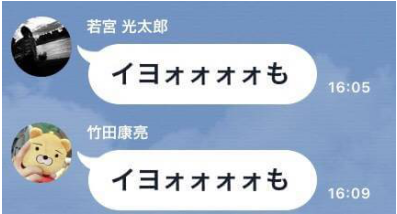
\includegraphics[clip,scale=0.5]{iii}
    \caption{小川男葉集III}
    \label{iii}
\end{figure}



\newpage
\subsubsection{小川男万葉集IV}
 \\
・アルステムダム\\
・オマンガンの鼻は犬\\
・広尾スタバ店\\
・スンマヒーンバッキンゴヒャクエンニナリマフー(交渉の余地なし)\\
・これで窪田美沙に投票するんやでぇトイレ\\
・公開固形(あつむ)\\
・なんかなああ(サイリウム)\\
・それではチェキのカウントダウンを始めます。5.4\\
    (2000円握りしめて)時間を止める\\
・結婚安泰 将来おめでとう\\
・非常に濃ゆい旅行であった\\
・インジビリブル\\
・次、オ・ガンマンのパアアン(ターン)\\
・シビリア鉄道\\
・よし。   \ \      え?\\
・まろやかさってパロメーター\\
・なにこのケンリツ(建立)\\
・タマンダンまだおるのかぁ(ATM)\\

\newpage
\subsubsection{小川男万葉集V}
・ミドルネーム何個あんの?\\
・あ、おれこの写真知らんわ(写っている)\\
・おれミツやわ、うぃ\\
・オガワポテンシャル、とうざい(到来)\\
・ひさやんバンバンビガロ(ひさやんレトリバー(レトリィバァ))\\
・山崎パルのハン祭(ポ)\\
・とうばらし(チェックイン)いや、軽い\\
・めっちゃ見たろう\\
・前田さんぶっ殺そう(ケータイ弄りながら)\\
・親指ちょっとでっかくして(Christoph Falk Anders)\\
・どういうモチベーションで生きたらいいん、差しコエ\\
・やすおこプンプン丸\\
・インストールできない実験にインストールできる(ティ)\\
・定量的には何もわかりません(ピ)\\
・本当にあってるかどうかはわからないんですが(ポ)\\
・擬ラピデティに関しましては、私はちょっと(マ)\\
・前回と比べると誤差は大きく小さくなったと言えます(マ)\\
・ペットボトル加速器\\
・パーラー\\
・ミートボール10個で100倍\\
・僕ミートボール\\
・1/16通り\\
・美容院には来週末で予定していたのでバサバサ頭が気になった。普段はもっと若々しくてハツラツとしてキレイにしてると友達に言っといてな\\


\newpage
\section{Clock Doraemon Threshold Valentien(CDTV)}
\subsection{オガワマワン(23)が結婚できない20の理由}
\subsubsection{オガワマワン(23)が結婚できない20の理由}
 \\
(1)収入が安定していない\\
(2)無職\\
(3)何かに追われている、余裕が無い\\
(4)休日はYouTubeを見ている\\
(5)地下アイドルに友達がいる\\
(6)4σを言い張る\\
(7)お酒が弱い\\
(8)財布を無くしがち\\
(9)芸人だから\\
(10)方向音痴だから\\
(11)Googleマップを使うのが下手くそ\\
(12)コンパイルがあんまり通らないあ\\
(13)希望新風が好きすぎる\\
(14)映画が好きじゃないから\\
(15)杉下右京が好きだから\\
(16)お腹が緩い\\
(17)ツッコミ過ぎる\\
(18)指が太い\\
(19)結婚指輪の制度を知らない\\
(20)結婚の意識が無い\\
(21)ボインボイン物語で喜ぶ\\
(22)天然だから\\
(23)土下座できない\\
\\
【説明】\\
この男はノリピーをこきおろしている。\\

\newpage
\subsubsection{オガワマワン(24)が結婚できない20の理由が冤罪である理由}
 \\
(1)社会人であるため安定している{\sf (´\_ゝ`)}笑\\
(2)社会人であるため無職ではない{\sf (´\_ゝ`)}笑\\
(3)追われていない、毎日工場実習で退屈な日々を過ごしている{\sf (´\_ゝ`)}笑\\
(4)そこまで見ていない、平日のほうが見ている{\sf (´\_ゝ`)}笑\\
(5)まあ知り合いといったところでしょうか{\sf (´\_ゝ`)}笑\\
(6)まあ5σ{\sf (´\_ゝ`)}笑\\
(7)弱いが嫌いではない{\sf (´\_ゝ`)}笑\\
(8)あれ以降なくしていない{\sf (´\_ゝ`)}笑\\
(9)芸人ではない{\sf (´\_ゝ`)}笑\\
(10)気のせい{\sf (´\_ゝ`)}笑\\
(11)Googleマップがバグっていただけ{\sf (´\_ゝ`)}笑\\
(12)コンパイルとか懐かしいな{\sf (´\_ゝ`)}笑\\
(13)海苔が好きなだけ{\sf (´\_ゝ`)}笑\\
(14)映画が好きじゃないわけではなく見る機会がないだけ{\sf (´\_ゝ`)}笑\\
(15)杉下右京が好きでもない{\sf (´\_ゝ`)}笑\\
(16)寒いのが悪い{\sf (´\_ゝ`)}笑\\
(17)ボケが多いだけ{\sf (´\_ゝ`)}笑\\
(18)指が太いとは思わない{\sf (´\_ゝ`)}笑\\
(19)制度とかあったっけ{\sf (´\_ゝ`)}笑\\
(20)ある{\sf (´\_ゝ`)}笑\\
(21)喜んだ記憶はない{\sf (´\_ゝ`)}笑\\
(22)天然ではない{\sf (´\_ゝ`)}笑\\
(23)できないことはない{\sf (´\_ゝ`)}笑\\
\\
【説明】\\
なんやこれ{\sf (´\_ゝ`)}笑\\


\newpage
\subsection{インビジブル天然巨乳である10の理由}
\begin{enumerate}
\item 財布を無くしたと喚き、2時間友人を捜索に付き合わせた結果、カバンから出てきた。
\item カードの1/19という使用期限の表記を見て、「平成19年1月」と記入した。
\item 極度の肩凝り。
\item macとディスプレイを繋いでいないのに、ディスプレイ側にポインターを持っていこうとしていた。
\item「旅費申請が出来ない! なんやねん、これ!」と憤っていたのに、実はパスワードの打ち間違いが原因であった。
\item 店長になろうとした
\item CERN出張の宿について話している時に「結局ホステスになりそう」と言った
\item ビジブル貧乳
\item 六甲道集合なのに、六甲に集合した。
\item macとディスプレイを繋いでいないのに、「いや、放電っぽい波形が」とほざき、ディスプレイ側にスライドを持っていこうとしていた。
\item 食器用洗剤と勘違いをして、オリーブオイルで食器を洗っていた。
\item 自らのオリーブオイルの過ちを、他人の過失として男葉集内で処理しようとした。
\end{enumerate}

\newpage
\subsection{理想の女性100の条件}
 \\
---------- 検索結果 ---------- \\
    澁川 ◯◯ *******  80\%\\
    横山 Yumi ******  10\%\\
    明石家さんま *** 10\%\\
    あき竹城 *********  1‰\\
---------------------------------\\
(1)性別が女\\
(2)日本人またはインド人\\
(3)性格が素晴らしい(自分の事をヨイショする)\\
(4)年齢は±5歳\\
(5)身長は0cm以上170cm以下\\
(6)お喋り(他愛もない会話ができる、まぁ喋らんくても良いんやけどな)\\
(7)オシャレ\\
(8)漢検4級以上持ってると良い\\
(9)センター試験も受験していると尚良い\\
(10)関西弁を喋ってくれると、萌える\\
(11)標準語は、イラッとする(そんな事無い)\\
(12)運動はできたほうが良い\\
(13)できれば陸上(そんな事は無い)\\
(14)できれば水泳(そんな事は無い)\\
(15)髪型は不問とする。髪質は要相談。\\
(16)貧乳  (A以下もしくはB以上)\\
(17)**体重カット**山崎さんより越智さん(強いて言うなら)\\
(18)**女優カット** 綾瀬はるか、石原さとみ以外(別に省いてもええよ)\\
(19)新垣結衣(まぁまぁまぁ)\\
(20)明石家さんま以外\\
(21)笑っている時、口を開いている(笑顔がステキ)\\
(22)歌唱力は和田アキ子以上、出来れば声量も和田アキ子\\
(23)メガネを掛けていないのが好ましい(あき竹城)\\
(24)タバコを吸わない\\
(25)体重は80kg以下\\
(26)ショートの方が良い(似合ってたら何でも良いけど)\\
(27)メンヘラ・束縛系は駄目(おれは束縛せぇへんから)\\
(28)大食いが好ましい\\
(29)山崎さんよりさんま\\
(30)徳永英明より高音域を歌える女性\\
(31)料理は好きで、自分よりちょっと上(パスタマシン保有)\\
(32)白い\\
(33)毛量は多いほうが好ましい、葉加瀬太郎\\
(34)Zカップ以下\\
(35)性格について俺から言うことは無い、ニートでも可\\
(36)脚が100cm、胴体60cm\\
(37)得意料理は和食であれば良い、スパイスの効いたカレーなら尚良。\\
(38)専業主婦でドM、首輪で飼いたい。\\
(39)早起き(4時起き)が良い\\
(40)インド\\
\\
-- reserved --\\ 
(65)チュエンティフォー\\
(80)胸が盆地\\
(89)未婚が望ましい\\
(100)自分の事がチュキダカラ(自分っておれやで)\\

\newpage
\subsection{オ・マンガンが女々しい10の理由}
\begin{enumerate}
\item 星野源が好きだから(アボカドはそこまで。)
\item .
\item .
\item .
\item .
\item .
\item .
\item .
\item .
\item .
\end{enumerate}


\subsection{オ・マンガンが男らしい10の理由}
\begin{enumerate}
\item .
\item .
\item .
\item .
\item .
\item .
\item .
\item .
\item .
\item .
\end{enumerate}

\newpage
\subsection{オ・マンガンがインド人かもしれない10の理由}
\begin{enumerate}
\item 顔がインド人(登校してすぐの発言)
\item 学部時代に英語でカバディを習得した。
\item 本名がガワッシュ・モハンマド
\item 好きなタイプがインド人
\item 牛より豚を食べる
\item タバコよりうんこ
\item ナマステ、と声を掛けられた。
\item .
\item .
\item .
\end{enumerate}

\subsection{オ・マンガンが前田健太かもしれない10の理由}
\begin{enumerate}
\item マエケン体操が上手い
\item .
\item .
\item .
\item .
\item .
\item .
\item .
\item .
\item .
\end{enumerate}

\newpage
\subsection{比叡比叡推進協会}
図\ref{gas1}に一覧を示す。

\begin{table}[htb]
\newcolumntype{C}{>{\centering}p{5em}}
\begin{center}
\begin{tabular}{|c|c|} 
\hline
	会長 & 小川圭将\tabularnewline  \hline
庶務 & 山下達郎\tabularnewline  \hline
東京支部長・人事部長 & 前川光輝\tabularnewline  \hline
幹事・忘年会隊長 & 越智敦彦\tabularnewline  \hline
補佐 & 藏重久弥\tabularnewline  \hline
環境保全対策長 & 小川圭将\tabularnewline  \hline
副総理 & 又吉硬木\tabularnewline  \hline
エンジニアリング部門隊長 & 村上ショージ\tabularnewline  \hline
環境保全部門 農園部隊隊長 & 小川圭将\tabularnewline  \hline
環境保全アセスメント部隊 & 解散\tabularnewline  \hline
失言訂正担当大臣 & 小川圭将\tabularnewline  \hline
迷子担当大魔王 & 小川圭将\tabularnewline  \hline
長野支部スキー本部長 & ニセヨンテ\tabularnewline  \hline
路面凍結防止部隊 & 若宮光太郎\tabularnewline  \hline
美声部門オーケストラ学科 & 美輪明宏\tabularnewline  \hline
自衛自衛部門安全保障学科 & 桜井誠\tabularnewline  \hline
医療部門心電図工作隊長 & 越智敦彦\tabularnewline  \hline
学長部門学長 &武田廣\tabularnewline 
	\hline
	\end{tabular}
	\end{center}
	\caption{比叡比叡推進協会}  
	\label{gas1}
\end{table}

\newpage
\subsection{オガワマンのあだ名一覧}
\begin{itemize}
\item オマゲン(12/21)
\item オマガンメン
\item オマンギョンボン号
\item オガワン・バンバ・バン
\item オゲンマン
\item オマンゲン・ゴン
\item オマンゲン
\item オマンゲンゴンガングン
\item オガコウモン
\item オ・ヨンジュン
\item バラタン星人
\item オマンゲン源マン
\item オマンゲングンソクバン
\item 宮崎マン
\item オガワ3
\item オゾンマン
\item オズ
\item オズモ
\item オザワ
\item オマンゲンゴンガンバ
\item オザンギン
\item On the rock
\item オガンディー
\item オガァァァバン
\item 御万願寺
\item クルシウス小川
\item オマンゲン
\item 世界のオギャワ
\item オガワン星人
\item オガワン・バンバン・ビガロ
\item オガワン・オガワ
\item オガワン・ババン・バンバンバン
\item おがパイオン
\item おーゆー
\item 湯川
\item オガワン・ケノービー
\item オガワのマンメン
\end{itemize}

